\section{Umsetzung} \label{sec:umsetzung}
Mithilfe der Grundlagen aus Kapitel 2\ref{sec:grundlagen} wird nun erläutert, wie aus der Schaltung des EMI-Filters mithilfe der Auftrennung in eine Gegentakt - und eine Gleichtaktschaltung die Einfügedämpfung(engl. Insertion Loss, IL) berechnet wird. 

\subsection{Berechnung der Einfügedämpfung} \label{subsec:einfugedampfung}

Die ursprüngliche Schaltung wird in eine Gleich- und Gegentschaltung aufgetrennt. Dieses Prinzip ist eine gängige Methode, da so Symmetrien entstehen, welche vereinfacht werden können. Für die beiden Ersatzschaltungen, werden jeweils als Kettenmatrizen \ref{Kettenmatrix} gebildet. Diese bestehen widerum aus Kettenmatrizen der einzelnen Längs- und Querimpedanzen. Aus der Kettenmatrix für die Ersatzschaltbilder wird mithilfe der Streuparameter direkt die Einfügungsdämpfung berechnet. Kettenmatrizen werden durch eine Kaskadierung vorgenommen, dies entspricht im wesentlichen der Matrixmultiplikation. \\


\paragraph{Zusammenfassen der Schaltungen} \label{par:zusammenfassungSchaltung}
Folgendes Kapitel zeigt Schritt für Schritt auf, wie die gegebenen Schaltungen vereinfacht werden können. Zudem wird beschrieben welche Komponenten vernachlässigt werden können. Der erste Abschnitt behandelt die Gleichtaktschaltung und in einem zweiten Abschnitt wird die Gegentaktschaltung behandelt.

\paragraph{Gleichtaktschaltung}\label{para:zusammenfassungGleichtakt}
Abbildung \ref{fig:CMSchaltungOriginal} zeigt die Schaltung aus der Aufgabenstellung. 
\begin{figure}[H]
	\centering
	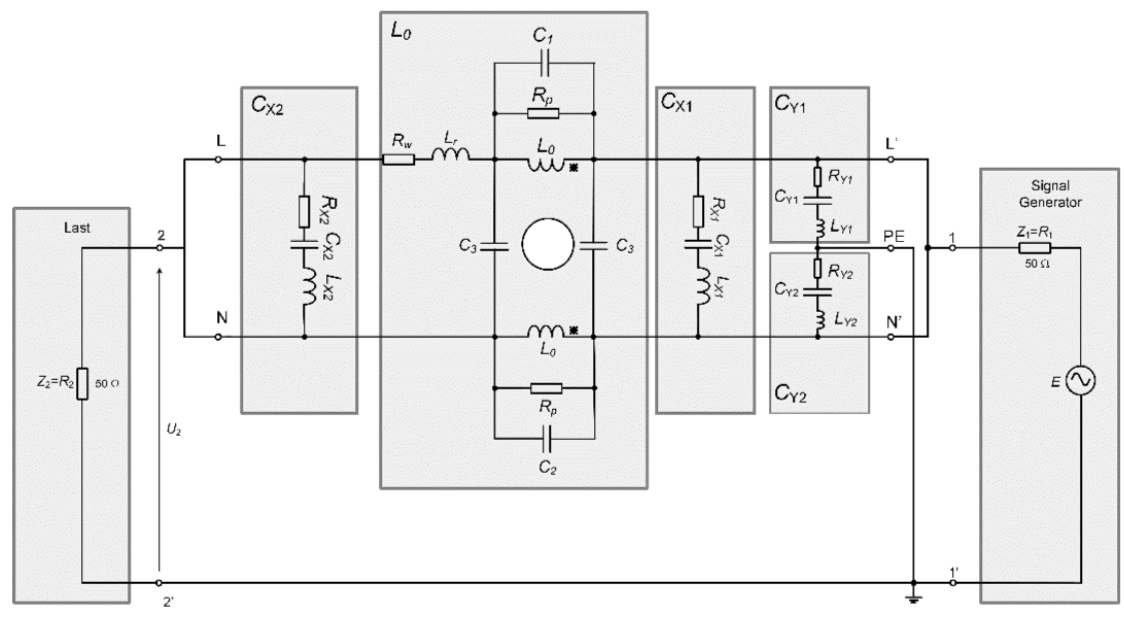
\includegraphics[width = 10cm]{CM_Aufgabenstellung.png}
	\caption{Originale Gleichtaktschaltung\cite{aufgabenstellung}}
	\label{fig:CMSchaltungOriginal}
\end{figure}
Die Originalschaltung ist mit den Komponenten $R_w$ und $L_r$ ergänzt worden, sodass sie symmetrisch ist(siehe Abbildung \ref{fig:CMSchaltungErgänzt}). Dies macht es möglich, dass die Schaltung zur Simulation wie folgt vereinfacht werden kann.
\begin{figure}[H]
	\centering
	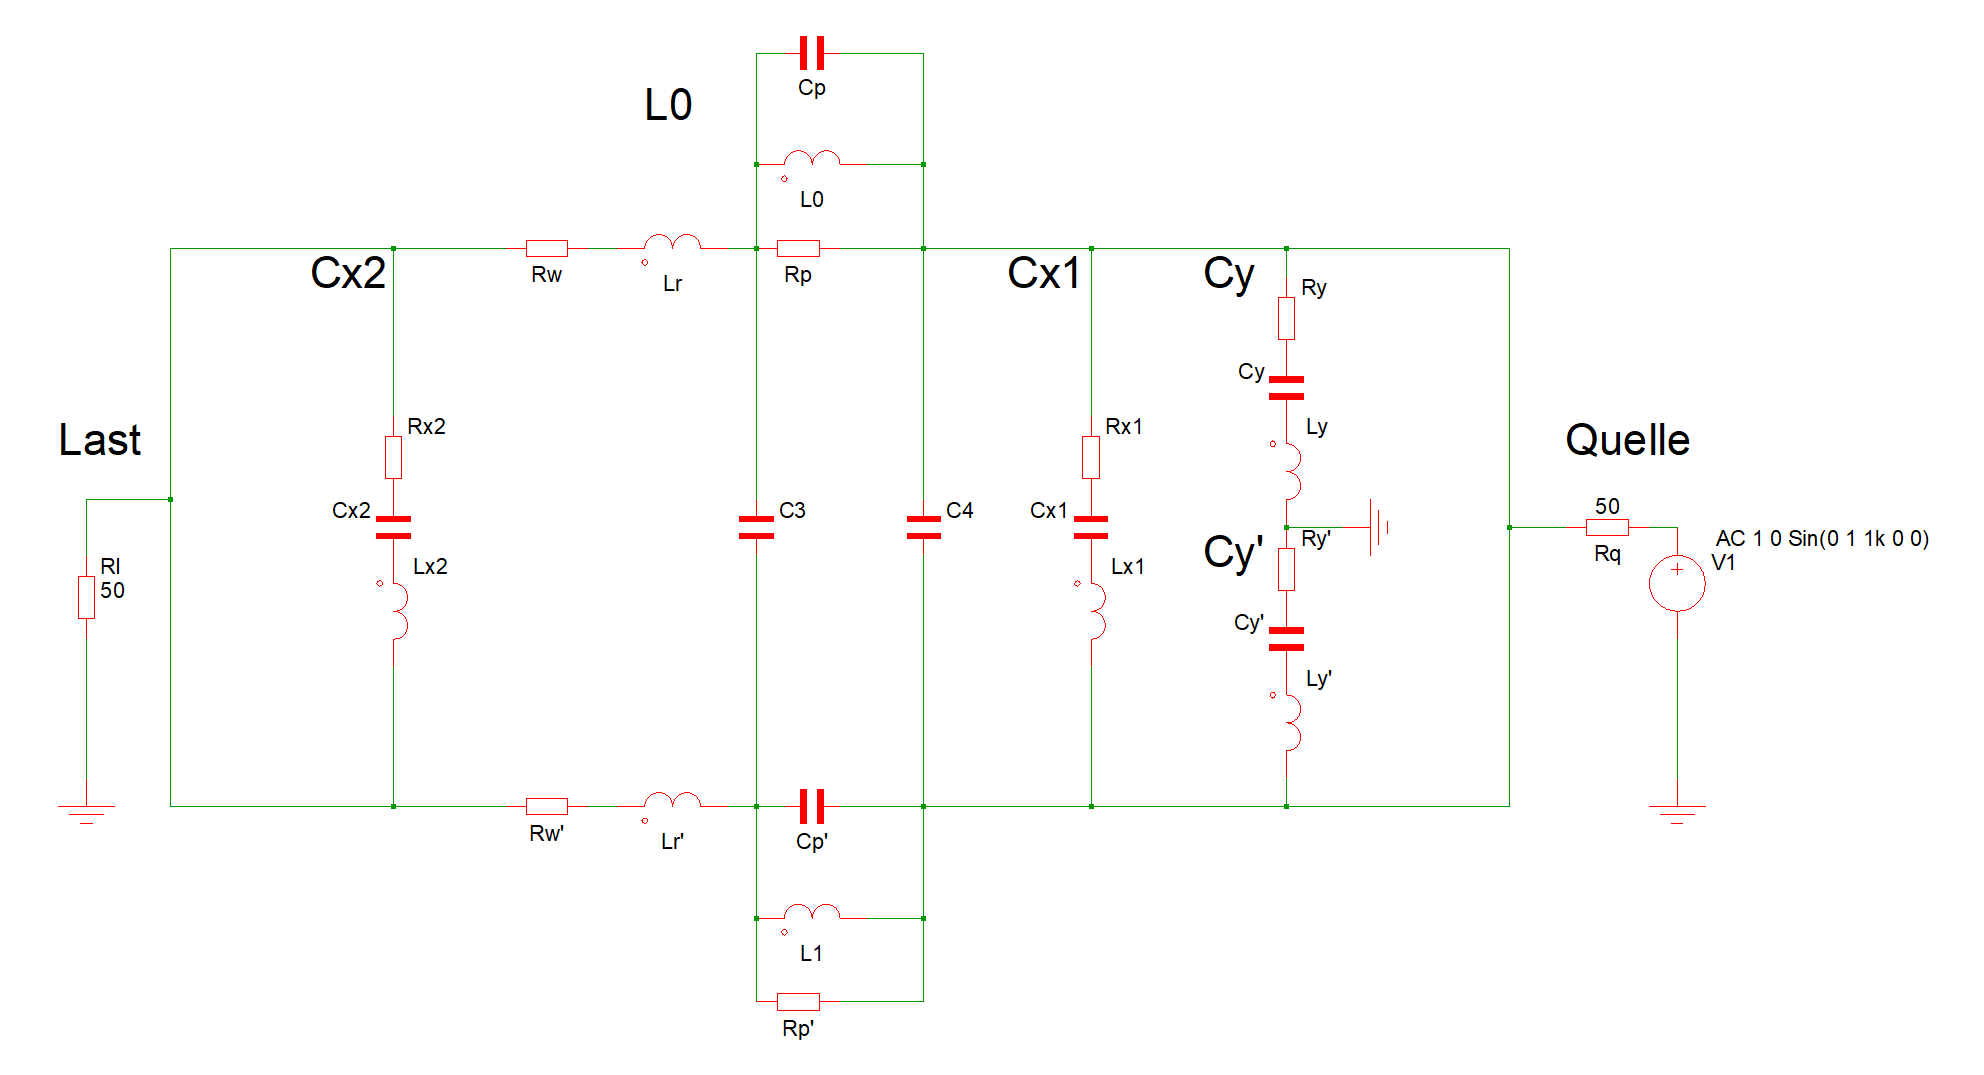
\includegraphics[width = 15cm]{EMI_CMpretty1.png}
	\caption{Ergänzte Gleichtaktschaltung}
	\label{fig:CMSchaltungErgänzt}
\end{figure}
Da der obere (siehe Abbildung \ref{fig:CMSchaltungErgänzt}, Nr. 1) und untere Strang (siehe Abbildung \ref{fig:CMSchaltungErgänzt}, Nr. 2) identisch sind und es keinen Potentialunterschied zwischen ihnen gibt, kann die Schaltung, wie folgt, zusammen gefasst werden (siehe Abbildung \ref{fig:CMSchaltungvereinfacht}). Die Schaltung wird entlang der Symmetrie-Achse (siehe Abbildung \ref{fig:CMSchaltungErgänzt}, Nr. 3) aufgetrennt. Somit fallen die Kondensatoren $C_3$, $C_4$, $C_{x1}$ und $C_{x2}$ komplett weg. Die übrigen Komponenten von $L_0$ bilden eine Parallelschaltung, welche sich durch halbieren der Widerstände und Induktivitäten und verdoppeln der Kapazitäten zusammenfassen lässt. Zusätzlich werden die beiden $C_y$ und $C'_{y}$ parallel auf das Bezugspotential geschalten. Da $C_y$ und $C'_y$ identisch sind, werden sie wie in Abbildung \ref{fig:CMSchaltungvereinfacht} zusammengefasst. Diese vereinfachte Schaltung bildet die Grundlage für die Berechnungen der Software.
\begin{figure}[H]
	\centering
	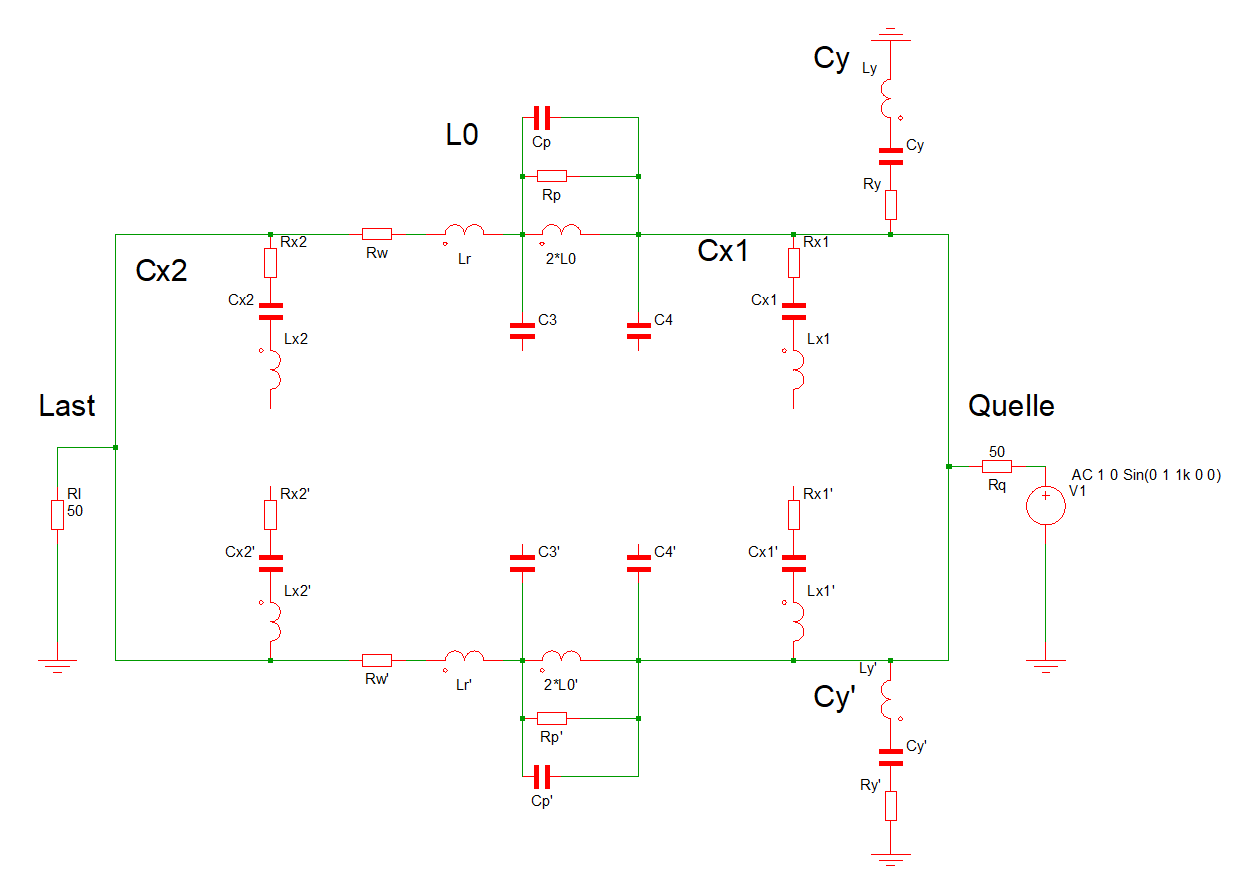
\includegraphics[width = 10cm]{EMI_CMpretty2.png}
	\caption{Vereinfachte Gleichtaktschaltung}
	\label{fig:CMSchaltungvereinfacht}
\end{figure}
\paragraph{Gegentaktschaltung}\label{para:zusammenfassungGegentakt}
Abbildung \ref{fig:DMSchaltungAufgabenstellung}
\begin{figure}[H]
	\centering
	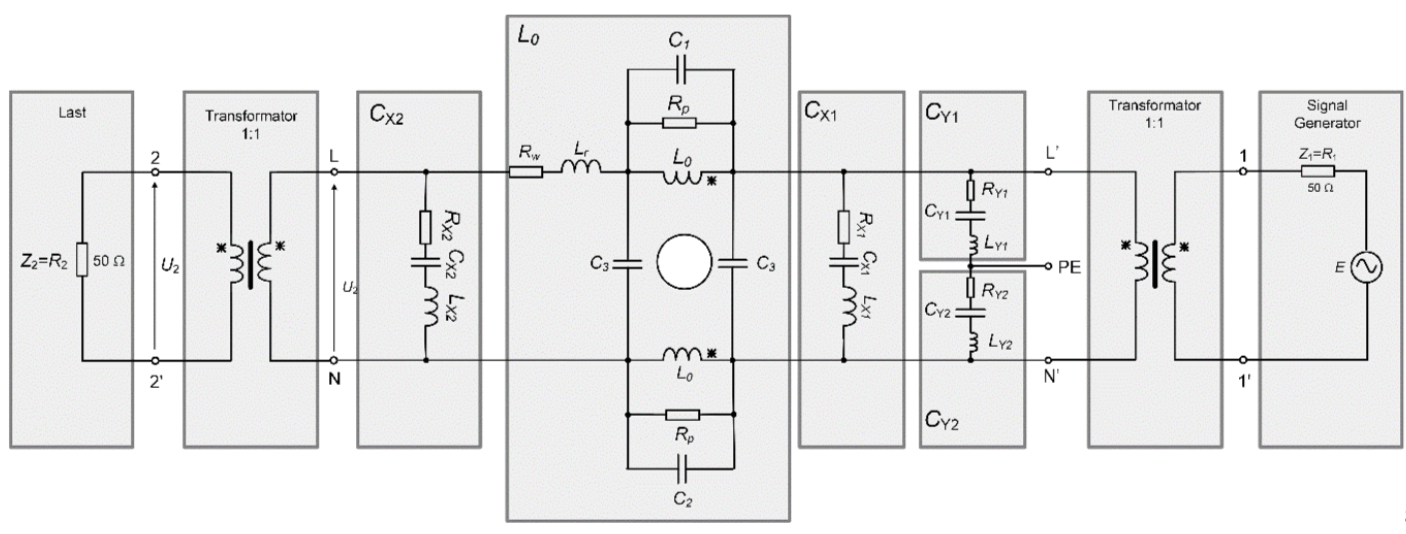
\includegraphics[width = 15cm]{DM_Aufgabenstellung.png}
	\caption{Ergänzte Gegentaktschaltung}
	\label{fig:DMSchaltungAufgabenstellung}
\end{figure}

%TODO fehlt noch?

Dieser Abschnitt fehlt noch


\paragraph{Rückwandlung} \label{par:ruckwandlung}

Die Kettenmatrizen führen dazu, dass die einzelnen Schaltungsteile entweder eine Längs-, oder eine Querimpedanz bilden müssen. Die Aufteilung der einzelnen Schaltungsteile in Längs- und  Querimpedanzen und ist in den Abbildungen (Verweis Aufteilung 1 und 2) grafisch dargestellt, wobei „LI“ eine Längsimpedanz kennzeichnet und „QI“ eine Querimpedanz.
\begin{figure}[H]
		\centering
		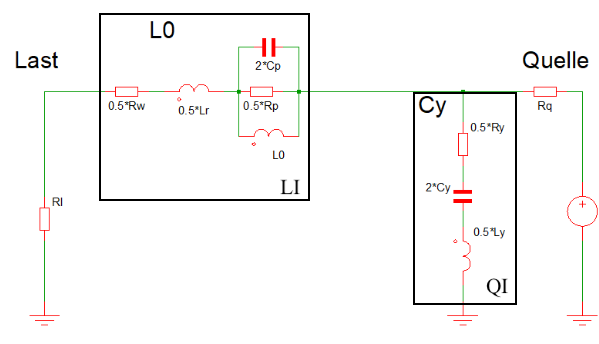
\includegraphics[width = 10cm]{EMI_CMvereinfacht_markiert.png}
		\label{fig:cmschaltung}
		\caption{Einteilung der Gleichtaktschaltungteile}
\end{figure}

\begin{figure}[H]
		\centering
		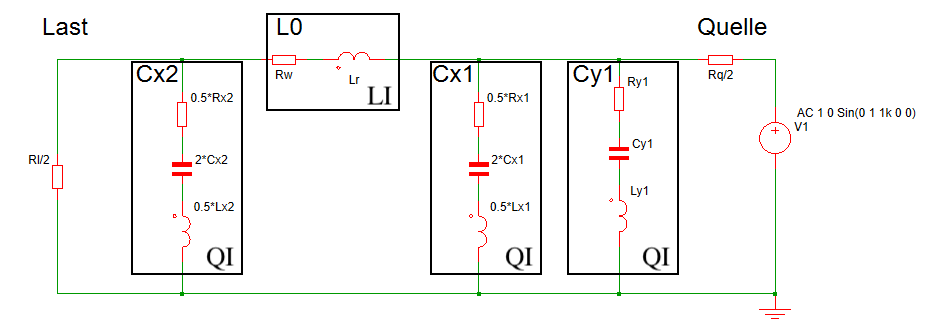
\includegraphics[width = 10cm]{EMI_DMvereinfacht_markiert.png}
		\label{fig:dmschaltung}
		\caption{Einteilung der Gegentaktschaltungsteile}
\end{figure}

Im nächsten Schritt werden die Impedanzen der einzelnen Schaltungsteile gebildet, welche in die passenden Kettenmatrizen eingesetzt werden.

\begin{equation}\label{equ:s21ausAMatrix}
s_{21} = \frac{2}{A_{11}+\frac{A{12}}{R_w}+A_{21}*R_w+A_{22}}
\end{equation}



Anhand der Kettenmatrizen der beiden Schaltungen, wird mit der Formel \ref{equ:s21ausAMatrix} der Streuparameter $S_{21}$ berechnet. A1 bis A4 entsprechen den einzelnen Einträge der Matrix. $R_w$ ist die Bezugsimpedanz. Die Bezugsimpedanz bezieht sich auf die Innenimpedanz der Quelle und die Lastimpedanz. Bezüglich der Aufgabenstellung(Verweis Aufgabenstellung) ist dieser auf 50Ohm festgelegt. Ausserdem ist es wichtig, dass die beiden Impedanzen gleich gross sind damit die Schaltung Reziprok ist (Verweis Theoretische Grundlagen: Reziproke Schaltungen). (Wieso ?) 
Bei der reduzierten Gegentaktschaltung (Abbildung \ref{fig:dmschaltung}) werden die beiden Impedanzen mit 25Ohm aufgeführt. Dies ergibt sich durch das Zusammenfassen der Gegentaktschaltung.\\


Die Berechnungen werden in MATLAB getätigt und geplottet. Diese Plots werden dann mit Simulationen in MPLAB Mindi verglichen um festzustellen ob diese korrekt sind. Nach überprüfung auf vollständikeit und korrektheit der Berechnungen, können diese in das Java implementiert werden. 